\section{Decision Tree}
Karar ağacı, bir veri setini, bir dizi karar uygulayarak daha küçük kümelere bölmek için kullanılan bir yapıdır. Karar ağacında ilk bölünmenin başladığı yere kök, dalların uzaması ile gelişen kısımlara düğüm, alt uçlara ise yaprak denir. Karar ağaçları, en iyi bölünmeyi seçmek için farklı kriterler kullanır. Daha uzun ağaçlar yerine daha kısa ağaçlar tercih edilir.  Düğümler:
\begin{enumerate}
    \item \textbf{Internal Node:} Özelliğin adı
    \item \textbf{Branch:} Bir üstteki özelliğin değeri
    \item \textbf{Leaf Node:} Tahmin Sınıfı
\end{enumerate}

\begin{figure}[h]
    \centering
    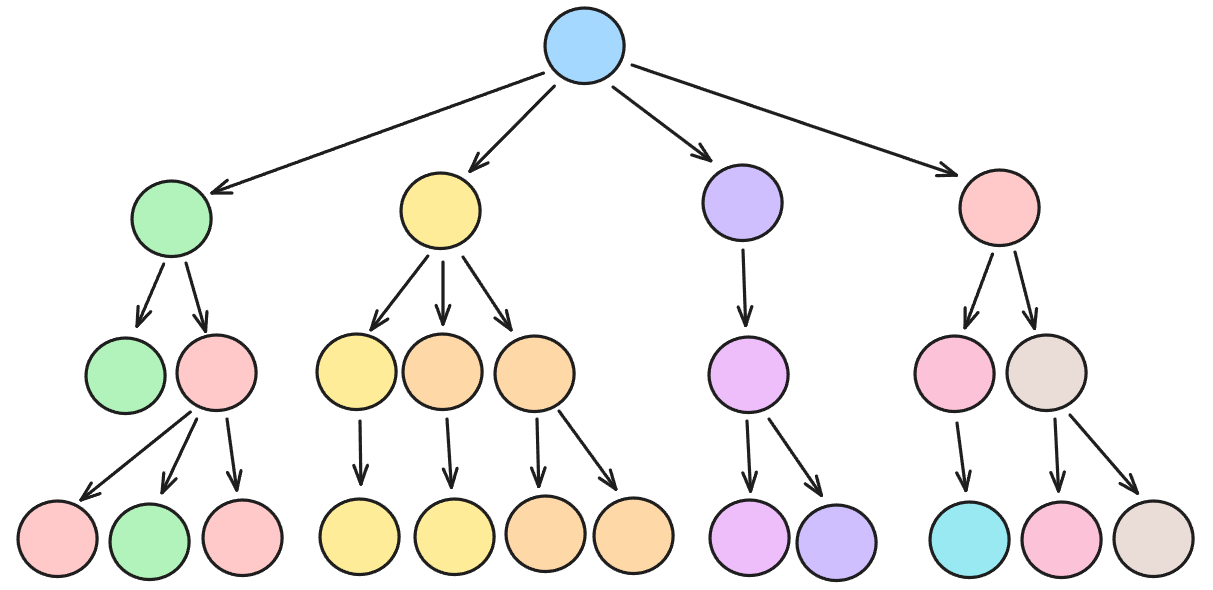
\includegraphics[width=1\textwidth]{images/decision_tree_structure.png}
    \caption{Karar ağacı.}
    \label{fig:enter-label}
\end{figure}

En yaygın olarak kullanılan algoritmalar.
\begin{enumerate}
    \item \textbf{Bilgi Kazancı (Information Gain):} Bir düğümün bölünmesinin ne kadar bilgi kazandıracağını ölçer. Bilgi kazancı, her alt düğümün belirli bir özellikle ne kadar homojen olduğunu gösteren bir metriktir. Bilgi kazancı, bir özellikle yapılan bölünmenin önceki duruma göre ne kadar daha az belirsizlik (bilgi eksikliği) getirdiğini ölçer. Bu, ağacın daha homojen alt gruplara bölünmesine ve iyi tahminler yapmasına yardımcı olur. Sırasıyla şu adımlar izlenir:
    \item \textbf{Entropi (Entropy):} Bir veri kümesinin ne kadar homojen veya heterojen olduğunu ölçen bir kavramdır. Daha yüksek entropi, daha fazla belirsizlik veya bilgi eksiliği anlamına gelir. Entropi şu formülle hesaplanır: E(S) = -p1 * log2(p1) - p2 * log2(p2) - ... - pk * log2(pk), burada p1, p2, ..., pk, S'deki her sınıfın olasılıklarıdır.
    \item \textbf{Dallanma (Split):} Bir özellik seçilir ve veri kümesi bu özelliğe göre alt gruplara bölünür. Her alt grup için entropi hesaplanır ve bu alt grupların ağırlıklı ortalaması (weighted average) alınır. Çok sayıda farklı kategorik değer alabilen özelliklerde Information Gain yöntemi etkili olmaz.
    \item \textbf{Jini Indeksi (Gini Index):} Bir düğümün homojenliğini ölçer. Daha küçük bir jini indeksi, daha homojen bir düğümü temsil eder.
\end{enumerate}

Pruning (Budama): Karar ağacında tahmine yeterince katkı yapmayan dallarda tahmin edici değişkenlerin modelden çıkarılması işlemidir. Post ve Pre olarak ikiye ayrılır. Prepruning, tahmin edici değişkenleri teker teker ele alarak modelin tahmin gücü için hangisinin etkili olacağı kararlaştırılarak adım adım dallanmaların ilerletilmesidir. Postpruning, tamamlanmış bir karar ağacından modele katkı yapmayan dalların tespit edilip modelden çıkarılmasıdır.

\subsection{Çalışma Adımları}
\begin{enumerate}
    \item Özellikler ve hedef değişken belirlenir.
    \item Ağacın kök düğümü seçilir ve veriler bu düğümde belirli bir özelliğe göre bölünür. Ardından, her alt düğüm için aynı adım tekrarlanır.
    \item Düğümler, en iyi bölünme kriterine göre alt düğümlere bölünür. Bölünme kriterleri genellikle bilgi kazancı, gini indeksi veya ortalama hata gibi metrikler kullanılarak belirlenir.
    \item Ağaç gereğinden fazla dallanma yapabilir. Bu nedenle gereksiz dallar kaldırılmaldır. (pruning)
    \item Yeni veriler için tahminler yapılır.
\end{enumerate}

\subsection{Avantajları}
\begin{enumerate}
    \item Yorumlaması kolaydır.
    \item Kullanılan ağaçlar görselleştirilebilir (sklearn.tree.plot\_tree()).
    \item Değişken seçimi yapabilir.
    \item Maaliyeti kullanılan veri boyutu ile logaritmiktir.
\end{enumerate}

\subsection{Dezavantajları}
\begin{enumerate}
    \item Overfitting sorunu. Budama işlemi ile önlenebilir.
    \item Heterojen veri üzerinde iyi performans göstermez.
    \item Yalnızca tek bir özellikle ilişkilendirilen ikinci sıra bağımlılıkları yakalayamaz.
\end{enumerate}

\newpage

\subsection{Hiperparametreler}
\begin{table}[h]
\centering
{\scriptsize\renewcommand{\arraystretch}{0.5}
{\resizebox*{\linewidth}{0.5\textwidth}{
\begin{tabular}{|p{3cm}|p{1cm}|p{1cm}|p{6cm}|}
\hline
Parametre & Type & Default & Açıklama \\ \hline
criterion & "gini", "entropy", "log\_loss" & "gini" & Ağaç oluşturma yöntemidir. \\ \hline
max\_depth & int & None & Ağacın maksimum derinliğini temsil eder. Değer verilmezse limitsiz olur. Overfitting'i önlemek için küçük bir değer girilmelidir. \\ \hline
min\_samples\_split & int/float & 2 & Bir düğümün bölünmeden önceki sahip olması gereken minimum örnek sayısıdır. \\ \hline
min\_samples\_leaf & int/float & 1 & Bir yaprağın sahip olması gereken minimum örnek sayısıdır. \\ \hline
min\_weight\_fraction\_leaf & float & 0 & Ağırlıklı örneklerin, toplam örnekler içerisindeki oranını temsil eder. \\ \hline
max\_leaf\_nodes & int & None & Maksimum yaprak sayısıdır. Overfitting'i engellemek için kullanılır. \\ \hline
max\_features & int/float, "auto", "sqrt", "log2" & None & En iyi bölünme için aranacak feature sayısıdır. \\ \hline

\end{tabular}
}}}
\end{table}

\newpage